%!TEX root = ../../master.tex
\subsection*{Experiment 1.2 - Tangible cloud cluster}

\subsubsection*{Module 1}
As described in the design of the experiment the first module included a votiee question on whether a cluster provided a better understanding of cluster computing after it had been demonstrated. The questions in the reflection did not cover the cluster since the students haven't used the cluster in Module 1. The results show that 15 out of 17 students thought it gave a better understanding.
\begin{figure}[H]
	\centering
	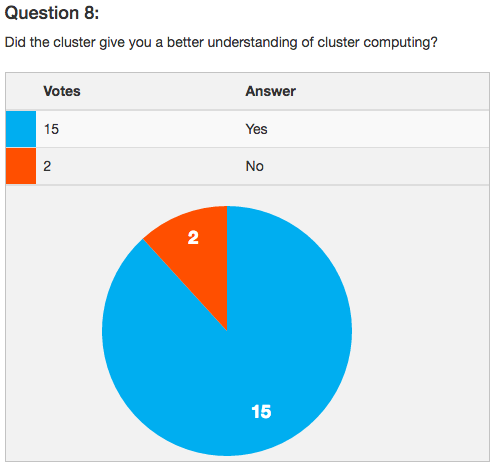
\includegraphics[width=6cm]{figures/appendix/cluster_understanding}
	\label{}
\end{figure}


\subsubsection*{Module 2 reflection}
The questionnaire from the second module contains one question regarding the tangible cloud computing cluster and if it helped the students' learning. The responses can be classified into different categories, as seen below.

\begin{itemize}
	\item Scale model (6/8)
	\item Helping learning (6/8)
	\item Not helping learning (2/8)
	\item Motivation (2/8)
\end{itemize}

\noindent The largest category was the Scale model which corresponds to Churchill's \textit{simulation object} which is a "representation of some real-life system or process". The cluster is e.g. referred to as a "remote host", "a small scale model" and "a device". \\
Six of eight students expressed, either directly or indirectly, that the cluster was a help e.g. because it visualized or illustrated something for them. Two students expressed that it did not help them. They point out that it could have been done without the cluster, and that it will be more clear when Kubernetes is introduced. These points are very valid, and the reason for having them use the cluster in this week was a preparation step towards the next week with Kubernetes. \\
Motivation is mentioned and backed up with that something was "cool" links to Piaget's emphasis of play and Hein's emphasis on motivation.

\renewcommand*{\arraystretch}{1.6}
\scriptsize
\begin{longtable}{|p{0.3cm}|p{14.7cm}|} 
\hline
\rowcolor[HTML]{EFEFEF} & \textbf{Question 5: Describe how (if) the Raspberry Pi Cluster helped your learning}  \\
\hline
\endfirsthead
\multicolumn{2}{c}%
{\tablename\ \thetable\ -- \textit{Continued from previous page}} \\
\hline
\rowcolor[HTML]{EFEFEF} &\textbf{Question 5: Describe how (if) the Raspberry Pi Cluster helped your learning}  \\
\hline
\endhead
\hline \multicolumn{2}{r}{\textit{Continued on next page}} \\
\caption{Question 5: Describe how (if) the Raspberry Pi Cluster helped your learning}
\endfoot
\caption{Question 5: Describe how (if) the Raspberry Pi Cluster helped your learning}
%\label{antipatterns}
\endlastfoot

1 & It helped me to know how to deploy a spring boot app to a remote host. \\ \hline 
2 & It haven't helped me much with the learning yet but i believe it will be more clear when we start working with kubernetes ;-) \\ \hline 
3 & Når vi allerede har gang i virtualisering og docker instancer, kunne man sagtens have undværet clusteret i forbindelse med dette moduls læring. \\ \hline 
4 & Its a working example and a small scale model \\ \hline 
5 & It definitely did, it made me see how cool it was to have the container running the JVM, and not having to host a guest OS on the raspberry, not even sure that would be a possibility. Even though it did take a while to make the image it was still cool to see it work on something else than your own machine, it demystified some of the "mystery" that's Docker. \\ \hline 
6 & The Cluster gives a real-time picture of working services. It is motivation to see your work do the things it is meant to do on a device \\ \hline 
7 & helped visualize a small server setup \\ \hline 
8 & The cluster illustrated how a service contained inside a docker container allows for deployment on a "low level" hardware ARM architecture.  \\ \hline  
\end{longtable}
\normalsize


\subsubsection*{Module 3 reflection}

The questionnaire from the third module contains four questions about whether or not the cluster helped the students’ learning. The responses can be classified into different categories, as seen below. \\

\noindent Question 3 contained an empty response. This response will not be counted in the sum of category responses below. The responses can be categorized in the following way.

\begin{itemize}
	\item Helping (7/7)
	\item Visualization (7/7)
	\item Location of pods (4/7)
\end{itemize}

\noindent
All students, except the empty answer, reported that the cluster helped their learning. The help from the visualization was mentioned in all the responses, and the location of the pods was also mentioned in different ways. The importance of the visualization is in agreement with Felder and Silverman's research on learning styles in which visual learning is preferred over verbal learning for most learners of college age and up.

\renewcommand*{\arraystretch}{1.6}
\scriptsize
\begin{longtable}{|p{0.3cm}|p{14.7cm}|} 
\hline
\rowcolor[HTML]{EFEFEF} & \textbf{Question 3: Describe how (if) the Raspberry Pi Cluster helped your learning}  \\
\hline
\endfirsthead
\multicolumn{2}{c}%
{\tablename\ \thetable\ -- \textit{Continued from previous page}} \\
\hline
\rowcolor[HTML]{EFEFEF} &\textbf{Question 3: Describe how (if) the Raspberry Pi Cluster helped your learning}  \\
\hline
\endhead
\hline \multicolumn{2}{r}{\textit{Continued on next page}} \\
\caption{Question 3: Describe how (if) the Raspberry Pi Cluster helped your learning}
\endfoot
\caption{Question 3: Describe how (if) the Raspberry Pi Cluster helped your learning}
\label{table:appendix_tangible_m3_q3}
\endlastfoot

1 & I think the Raspberry Pi cluster (as well as the visualizer) helped me to understand how Kubernetes works and where the different deployments were located and what happened if we pulled the network cable in one of the machines. \\ \hline 
2 & The cluster illustrates the purpose and setup visually in a nice way. It is very hands on to work with these compared to some cloud setup where the actual servers in the cluster are hidden away. \\ \hline 
3 & . \\ \hline 
4 & It was great to visualize how the pods are arranged and how the rolling release exchanged them \\ \hline 
5 & It definitely helped visualize the concept of the kubernetes cluster. The terminal ui of kubernetes is of course good as is, but the visualization (k8s-visualizer) was a big help to understand the actual relations, which can be hard to see in the default kubernetes terminal ui. \\ \hline 
6 & The clusters working as node + the visualization tool helped alot seeing how the scaling worked, and what effect it had on the system. \\ \hline 
7 & The raspberry pi, together with the kubernetes visualizer helped my learning by showing graphically how more replicas of containers are deployed to multiple pi's and how the update phase from a version to another was going on. \\ \hline 
8 & Helps visualize how a server could break Down and how kubernetes would restore the services else where \\ \hline 
\end{longtable}
\normalsize

% Question 4
\noindent The answers for Question 4 are similar to Question 3, and some of the students say that they already have answered it in the previous question. Similar to "Visualization" from Question 3 is the category "Overview" in Question 4 in which the Kubernetes concepts and overview is understood.

\renewcommand*{\arraystretch}{1.6}
\scriptsize
\begin{longtable}{|p{0.3cm}|p{14.7cm}|} 
\hline
\rowcolor[HTML]{EFEFEF} & \textbf{Question 4: Describe how the Kubernetes visualization tool helped your learning}  \\
\hline
\endfirsthead
\multicolumn{2}{c}%
{\tablename\ \thetable\ -- \textit{Continued from previous page}} \\
\hline
\rowcolor[HTML]{EFEFEF} &\textbf{Question 4: Describe how the Kubernetes visualization tool helped your learning}  \\
\hline
\endhead
\hline \multicolumn{2}{r}{\textit{Continued on next page}} \\
\caption{Question 4: Describe how the Kubernetes visualization tool helped your learning}
\endfoot
\caption{Question 4: Describe how the Kubernetes visualization tool helped your learning}
\label{table:appendix_tangible_m3_q4}
\endlastfoot

1 & Instead of running "kubectl get pods" command high frequently, it was a big help that you could see which containers was terminating, running and pending Live updated. \\ \hline 
2 & Answered in previous question \\ \hline 
3 & I provides a nice overview on the system status. I don't think there is so much learning in it, but the overview is nice when setting things up. \\ \hline 
4 & It gave a good idea how things are connected, and how replication works \\ \hline 
5 & The visualization tool is a bit slow. But it is always nice to see that what you are doing has an impact. The GUI of the tool gives an easy to understand overview of the system \\ \hline 
6 & Erhm, this was answered in question 3, i believe. " The terminal ui of kubernetes is of course good as is, but the visualization (k8s-visualizer) was a big help to understand the actual relations, which can be hard to see in the default kubernetes terminal ui. " \\ \hline 
7 & Together with the cluster it gave a very good picture of how kubernetes work both without and with server failure \\ \hline 
8 & Pretty much the same and the pi cluster \\ \hline 
9 & It helped me to understand where deployments were located and which services that were stated. 

	\noindent Another cool part of the visualizer is that it were easy to see what happened when Kubernetes were asked to scale the deployments. \\ \hline 
\end{longtable}
\normalsize


% Question 5
\noindent
Question 5's responses show that four students either did not see it as a help or did not understand the scheduling happening in the cluster. Three students understood that the pods are being scheduled on the Raspberry Pis in front of them.
\begin{itemize}
	\item A help (3/7)
	\item Not a help (4/7)
\end{itemize}

\renewcommand*{\arraystretch}{1.6}
\scriptsize
\begin{longtable}{|p{0.3cm}|p{14.7cm}|} 
\hline
\rowcolor[HTML]{EFEFEF} & \textbf{Question 5: How did the cluster help you understand the scheduling done by Kubernetes?}  \\
\hline
\endfirsthead
\multicolumn{2}{c}%
{\tablename\ \thetable\ -- \textit{Continued from previous page}} \\
\hline
\rowcolor[HTML]{EFEFEF} &\textbf{Question 5: How did the cluster help you understand the scheduling done by Kubernetes?}  \\
\hline
\endhead
\hline \multicolumn{2}{r}{\textit{Continued on next page}} \\
\caption{Question 5: How did the cluster help you understand the scheduling done by Kubernetes?}
\endfoot
\caption{Question 5: How did the cluster help you understand the scheduling done by Kubernetes?}
\label{table:appendix_tangible_m3_q5}
\endlastfoot

1 & Physically you had 4 devices you could deploy to instead of virtual machines. And by 4 devices I could see how kubernetes scheduled new replicas on the cluster, instead of vm's or in a terminal. \\ \hline 
2 & It showed how the pods were distributed among the pi's \\ \hline 
3 & Im not sure it did \\ \hline 
4 & . \\ \hline 
5 & I don't understand the scheduling done, at the moment. \\ \hline 
6 & Also answered in question 3. The cluster and the raspberries running as nodes in a cluster helped seeing how "unplugging" or upgrading worked. \\ \hline 
7 & not really sure. \\ \hline 
8 & Pass \\ \hline 

\end{longtable}
\normalsize

% Question 7
\noindent
Question 7 revealed that three of the students liked that it was "hands on" or a practical application of the theory. The workshop format was both supported and criticized. The drawback of four students sharing a cluster was pointed out by one student, who did not think the observing students got as much out of it as the "person who actually sat at the pc". This illustrates an interesting point of view when you look at mediating tools from activity theory. The students (subjects) has the goal (object) of learning about cluster management and Kubernetes. To reach this goal the cluster acts as a mediating tool. The previous statement underlines the importance of this tool, since it is not equally available for all members of the group. The workshop was both criticized and commended, whic shows a disagreement between the students.
 
\renewcommand*{\arraystretch}{1.6}
\scriptsize
\begin{longtable}{|p{0.3cm}|p{14.7cm}|} 
\hline
\rowcolor[HTML]{EFEFEF} & \textbf{Question 7: How did the workshop help you understand this week's topic?}  \\
\hline
\endfirsthead
\multicolumn{2}{c}%
{\tablename\ \thetable\ -- \textit{Continued from previous page}} \\
\hline
\rowcolor[HTML]{EFEFEF} &\textbf{Question 7: How did the workshop help you understand this week's topic?}  \\
\hline
\endhead
\hline \multicolumn{2}{r}{\textit{Continued on next page}} \\
\caption{Question 7: How did the workshop help you understand this week's topic?}
\endfoot
\caption{Question 7: How did the workshop help you understand this week's topic?}
\label{table:appendix_tangible_m3_q7}
\endlastfoot

1 & hands on is the best learning tool \\ \hline 
2 & Hands on is all ways good. I do think that the overview in the workshops can become a bit blurred.

	\noindent It provides much of a step by step approach which "any one" can do. This can become a weakness in the learning process.
	
	\noindent If each goal in a workshop was more clear and some subtle hints to lead the way, was used, I think they would be more rewarding. \\ \hline 
3 & The workshop was very well written, and informative. Keep up the good guides! \\ \hline 
4 &  I helped me a lot since it provided all the central commands for Kubernetes which should otherwise have been looked up in the documentation.
	
	\noindent A thing that I would have preferred were a more project oriented approach (or a part dealing with that) since we were kind of lost on how to configure our project such that it would be able to run using Kubernetes.
 \\ \hline 
5 & Easy to understand-easy to work on. But it is hard being 4 in a group on all work on it at the same time with 1 cluster. The workshop seems to be designed for 1 person doing it at a time. But because of the cluster limitations 4 persons was doing it on 1 pc on 1 cluster. I think the person who actually sat at the pc was the person who got most out of the workshop \\ \hline 
6 & It gave me a platform to scratch the surface of kubernetes, i definitely do not feel like a pro, and as i sit here writing this i don't remember half the commands that i used to launch everything, but it did provide a good basis, and using the pi cluster is a nice addition to running it locally. \\ \hline 
7 & practical application of the teory \\ \hline 
8 & It's hard to tell. It seems like there is a great step between the workshops and the actual project work. \\ \hline 
9 & It did a great deal. A lot of the steps you had to follow gave a little bit of extra knowledge, instead of getting a huge information overload when you then had to remember, The Kubernetes workshop also felt alot more complete than the Docker one, where I personally did not learn that much. \\ \hline 
\end{longtable}
\normalsize





\subsubsection*{Module 4 reflection}
TBD FIX!


%%%%% Q4
\renewcommand*{\arraystretch}{1.6}
\scriptsize
\begin{longtable}{|p{0.3cm}|p{14.7cm}|} 
\hline
\rowcolor[HTML]{EFEFEF} & \textbf{Question 4: Describe how (if) the Raspberry Pi Cluster helped your learning}  \\
\hline
\endfirsthead
\multicolumn{2}{c}%
{\tablename\ \thetable\ -- \textit{Continued from previous page}} \\
\hline
\rowcolor[HTML]{EFEFEF} &\textbf{Question 4: Describe how (if) the Raspberry Pi Cluster helped your learning}  \\
\hline
\endhead
\hline \multicolumn{2}{r}{\textit{Continued on next page}} \\
\caption{Question 4: Describe how (if) the Raspberry Pi Cluster helped your learning}
\endfoot
\caption{Question 4: Describe how (if) the Raspberry Pi Cluster helped your learning}
\label{w4_q4}
\endlastfoot

1 & same as the workshop aswer \\ \hline

2 & The cluster is great at getting down to earth on the understander of clusters and the error scenarios present in such systems. \\ \hline


3 & helped provide some low power servers to load test on. and the possibility to "pull the plug" ;) \\ \hline


4 & It was very nice to be able to pull out network cables and see what happens. A good help \\ \hline


5 & It helped a lot. I were nice to see what actually happened when a machine were disconnected and how that affects the system. \\ \hline


6 & There was a physical object you could attack and a physical link you should unlink (Lan cable). This helped understading how a part of a system could be down, and other parts can take over the service. \\ \hline


7 & The cluster is a good abstraction of the pods, and how to make them unavailable by pulling the plug. \\ \hline


8 & because of the cluster we could physically pull a plug, that the system had to bounce back from. \\ \hline


\multicolumn{2}{r}{\textbf{Evaluation:} TBD} \\ 
\end{longtable}
\normalsize


%%%%% Q5
\renewcommand*{\arraystretch}{1.6}
\scriptsize
\begin{longtable}{|p{0.3cm}|p{14.7cm}|} 
\hline
\rowcolor[HTML]{EFEFEF} & \textbf{Question 5: Did the cluster support your understanding of what resilience is? If yes, how?}  \\
\hline
\endfirsthead
\multicolumn{2}{c}%
{\tablename\ \thetable\ -- \textit{Continued from previous page}} \\
\hline
\rowcolor[HTML]{EFEFEF} &\textbf{Question 5: Did the cluster support your understanding of what resilience is? If yes, how?}  \\
\hline
\endhead
\hline \multicolumn{2}{r}{\textit{Continued on next page}} \\
\caption{Question 5: Did the cluster support your understanding of what resilience is? If yes, how?}
\endfoot
\caption{Question 5: Did the cluster support your understanding of what resilience is? If yes, how?}
\label{w4_q5}
\endlastfoot

1 & didnt think it mattered much for the understanding on this topic \\ \hline

2 & yes as it allows to directly see the effects of errors simply by pulling a plug \\ \hline

3 & Somewhat, since the services could be started on another pi, if one of them crashed. \\ \hline

4 & Yes. Replicas of the app helped the understanding of how the "slaves" could help eachother when one was taken down. \\ \hline

5 & The pods and plugs makes for a good visualization. \\ \hline

6 & yes it did, by allowing to physically pull the plug and see the system recover. \\ \hline

7 & When able to manually take out a node in the cluster and watch the performance recover automatically, the possibilities are very straight forward. \\ \hline

8 & Absolutely. It showed how different mechanisms can be used to recover from errors and how kubernetes handles a disconnected machine. \\ \hline

9 & yes. It gave a good hands on experience to see that the kubernetes recovers by it self.  \\ \hline

\multicolumn{2}{r}{\textbf{Evaluation:} TBD} \\ 
\end{longtable}
\normalsize


\subsubsection*{Module 5 reflection}
TBD

\subsubsection*{Module 6 reflection}
TBD

\subsubsection*{Module 7 reflection}
TBD